\chapter[ANALYSE ET CONCEPTION DU SYSTÈME]{ANALYSE ET CONCEPTION DU SYSTÈME}
    \section[Introduction partielle]{Introduction partielle}
    Ce chapitre vise à offrir une vue d’ensemble sur l’analyse et une vue logique du
    système informatique qui sera développé. Dans le cycle de vie d’un système informatique,
    il existe deux étapes primordiales qui sont : l’analyse et la conception. L’analyse nous
    permet d’avoir une idée sur les besoins du travail. Il permet également d’avoir un aperçu
    du résultat. La conception, quant à elle, nous permet de décrire par un langage de
    modélisation de données (UML dans notre cas) la structure et le fonctionnement du
    système d’information.
        \section[Identification et représentation des besoins]{Identification et représentation des besoins}    
    \subsection[Identification des acteurs]{Identification des acteurs}
    Voici les acteurs identifiés dans le cadre de notre
    travail :
    \par
        \begin{itemize}
            \setlength{\itemsep}{0pt}
            \item [\ding{226}] \textbf{L’internaute} : est celui qui visite
            notre plateforme sans y être inscrit.
            \item [\ding{226}] \textbf{Le client} : est celui qui a créé un compte
            utilisateur dans le système.
            \item [\ding{226}] \textbf{L’administrateur} : il est chargé de
            monitorer le système afin d’éviter tout débordement des utilisateurs,
            et voir tous les mauvais fonctionnements du système et les régler
            à distance.
            \item [\ding{226}] \textbf{Le manager} : est celui qui utilise le système
            pour visualiser le tableau de bord et consulter le rapport.
        \end{itemize}
    \subsection[Identification des cas d’utilisation]{Identification des cas d’utilisation}
    Les cas d’utilisations ou fonctionnalités de notre
    système sont les suivants :
    \par
        \begin{itemize}
            \setlength{\itemsep}{0pt}
            \item [\ding{226}] Créer compte
            \item [\ding{226}] S’authentifier
            \item [\ding{226}] Afficher avis
            \item [\ding{226}] Afficher notification
            \item [\ding{226}] Valider jeton
            \item [\ding{226}] Donner avis
            \item [\ding{226}] Établir rapport
            \item [\ding{226}] Vendre billet
            \item [\ding{226}] Gérer compte
            \item [\ding{226}] Ajouter évaluation
            \item [\ding{226}] Génère tableau de bord
            \item [\ding{226}] Consulter tableau de bord
            \item [\ding{226}] Consulter rapport
        \end{itemize}
    Chacun des cas figurant dans la liste présenter
    ci-haut, seras expliquer plus en détaille dans
    sa description textuelle.
\pagebreak
    \subsection[Diagrammes de cas d’utilisation]{Diagrammes de cas d’utilisation}
    Après avoir eu à identifier les acteurs et leurs cas d’utilisation
    voici comment se présente le diagramme de cas d’utilisation :
        \begin{figure}[H]
            \centering
            
\includegraphics[width=150mm]{images/dcu_systeme.png}
            \caption{Diagramme de cas d’utilisation}
            \label{fig:dcu}
        \end{figure}
\pagebreak
        \section[Spécification détaillée des besoins]{Spécification détaillée des besoins}
Dans cette étape, nous allons détailler la description des besoins par la description textuelle
des cas d’utilisation et la production de diagrammes de séquence système
illustrant cette description textuelle. \cite*{audibert2008uml}  
    \subsection[Description textuelle des cas d'utilisation]{Description textuelle des cas d’utilisation}
        \subsubsection[Créer compte]{Créer compte}
            \begin{longtable}{p{4cm} p{9cm}}
                \caption{Description textuelle du cas d’utilisation Créer compte}
                \label{table:usecaseCreeCompte}
                \\\hline\hline
                    \textbf{Cas d’utilisation} & \textbf{Créer compte}
                \\\hline\hline
                        \textbf{Acteur principal} & L’\textsc{internaute}
                    \\
                        \textbf{Acteur secondaire} & -
                    \\
                        \textbf{Objectifs} & L’\textsc{internaute} veut être 
                        enregistré dans le système.
                    \\
                        \textbf{Préconditions} & -
                    \\
                        \textbf{Postcondition} & Un compte a était créé.
                    \\
                        \textbf{Scénario nominal} &
                            \begin{enumerate}[leftmargin=*]
                                \item L’\textsc{internaute} clique sur créer compte et le
                                système affiche un formulaire.
                                \item L’\textsc{internaute} saisi ses identifiants à savoir
                                (nom, post-nom, date et année de
                                naissance, âge et genre) et coordonnées (téléphone, adresse physique
                                et adresse électronique).
                                \item L’\textsc{internaute} confirme en cliquant sur créer.
                                \item Le système enregistre les nouvelles informations
                                dans la base de données et le
                                système répond avec un message de succès.
                            \end{enumerate}
                    \\
                        \textbf{Scénario alternatif} &
                            \begin{enumerate}[leftmargin=*]
                                \item À partir de l’étape numéro 3 du scenario nominal
                                le système vérifie et ne valide pas le formulaire
                                \item Retour à l’étape numéro 1 du scénario principal
                            \end{enumerate}
                \\\bottomrule
            \end{longtable}
            %\pagebreak

        \subsubsection[S’authentifier]{S’authentifier}
            \begin{longtable}{p{4cm} p{9cm}}
                \caption{Description textuelle du cas d’utilisation S’authentifier}
                \label{table:usecaseSauth}
                \\\hline\hline
                    \textbf{Cas d’utilisation} & \textbf{S’authentifier}
                \\\hline\hline
                        \textbf{Acteur principal} & L’\textsc{internaute}, le \textsc{client},
                        le \textsc{guichetier}, le \textsc{manager} et l’\textsc{administrateur}
                    \\
                        \textbf{Acteur secondaire} & -
                    \\
                        \textbf{Objectifs} & L’utilisateur veut accéder au système.
                    \\
                        \textbf{Préconditions} & -
                    \\
                    \textbf{Postcondition} & L’utilisateur a accès au système
                    \\
                    \textbf{Scénario nominal} &
                        \begin{enumerate}[leftmargin=*]
                            \item L’utilisateur saisis les informations de connexion à savoir (le mot de
                            passe et l’identifient).
                            \item Il confirme en cliquant sur le bouton se connecter.
                            \item Le système vérifie les informations saisies et crée la session.
                        \end{enumerate}
                    \\
                    \textbf{Scénario alternatif} &
                    \begin{enumerate}[leftmargin=*]
                            \item L’utilisateur annule la modification et le système revient sur l’interface de
                            connexion.
                        \end{enumerate}
                    \\
                    \textbf{Exception} &
                    \begin{enumerate}[leftmargin=*]
                            \item Le système détecte que les identifiants saisis sont incorrects et communique à
                            l’utilisateur que les informations saisies sont incorrectes sous forme d’erreur et
                            retourne à la page de connexion.
                        \end{enumerate}
                \\\bottomrule
            \end{longtable}

        \subsubsection[Consulter avis]{Afficher avis}
            \begin{longtable}{p{4cm} p{9cm}}
                \caption{Description textuelle du cas d’utilisation Afficher avis}
                \label{table:usecaseConsulterAvis}
                \\\hline\hline
                    \textbf{Cas d’utilisation} & \textbf{Afficher avis}
                \\\hline\hline
                        \textbf{Acteur principal} & L’\textsc{internaute} et le \textsc{client}
                    \\
                        \textbf{Acteur secondaire} & -
                    \\
                        \textbf{Objectifs} & L’\textsc{internaute} veut afficher les
                        avis des clients (commentaires et évaluations données)
                    \\
                        \textbf{Préconditions} & -
                    \\
                    \textbf{Postcondition} & L’\textsc{internaute} a lu les avis.
                    \\
                    \textbf{Scénario nominal} &
                        \begin{enumerate}[leftmargin=*]
                            \item L’\textsc{internaute} clique sur le bouton
                            voir avis.
                            \item Le système affiche les avis des clients.
                        \end{enumerate}
                    \\
                    \textbf{Scénario alternatif} &
                        \begin{enumerate}[leftmargin=*]
                            \item Le système est indisponible.
                        \end{enumerate}
                \\\bottomrule
            \end{longtable}

        \subsubsection[Afficher notification]{Afficher notification}
        \begin{longtable}{p{4cm} p{9cm}}
            \caption{Description textuelle du cas d’utilisation Afficher notification}
            \label{table:usecaseAfficherNotification}
            \\\hline\hline
                \textbf{Cas d’utilisation} & \textbf{Afficher notification}
            \\\hline\hline
                    \textbf{Acteur principal} & Le \textsc{client}
                \\
                    \textbf{Acteur secondaire} & -
                \\
                    \textbf{Objectifs} & Le \textsc{client} veut lire une
                    notification.
                \\
                    \textbf{Préconditions} & Le \textsc{client} s’est authentifié.
                \\
                    \textbf{Postcondition} & Le \textsc{client} a lu sa notification.
                \\
                \textbf{Scénario nominal} &
                    \begin{enumerate}[leftmargin=*]
                        \item Le \textsc{client} parcours la page d’accueil ;
                        \item Le système affiche une infobulle avec un numéro indiquant le nombre de
                        notifications ;
                        \item Le \textsc{client} clique sur la cloche de notification.
                        \item Le système affiche une boite de dialogue avec toutes les notifications.
                        \item Le \textsc{client} clique sur la notification voulue
                        \item Le système affiche les détails de la notification sélectionnée et décrémente le
                        nombre de notifications.
                    \end{enumerate}
                \\
                \textbf{Scénario alternatif} &
                    \begin{enumerate}[leftmargin=*]
                        \item Le système est indisponible.
                    \end{enumerate}
            \\\bottomrule
        \end{longtable}

        \subsubsection[Valider ticket]{Valider ticket}
        \begin{longtable}{p{4cm} p{9cm}}
            \caption{Description textuelle du cas d’utilisation Valider ticket}
            \label{table:usecaseScannerJ}
            \\\hline\hline
                \textbf{Cas d’utilisation} & \textbf{Valider ticket}
            \\\hline\hline
                    \textbf{Acteur principal} & Le \textsc{client}
                \\
                    \textbf{Acteur secondaire} & -
                \\
                    \textbf{Objectifs} & Le \textsc{client} veut vérifier la
                    validité de son ticket ticket de bus.
                \\
                    \textbf{Préconditions} & Le \textsc{client} s’est authentifié.
                \\
                    \textbf{Postcondition} & Le \textsc{client} a vérifié la validité de son ticket.
                \\
                \textbf{Scénario nominal} &
                    \begin{enumerate}[leftmargin=*]
                        \item Le \textsc{client} clique sur valider ticket dans
                        l’interface de \textsc{donner avis}
                        \item Le système affiche un formulaire de validation de ticket
                        \item Le \textsc{client} saisie le code du ticket et valide.
                        \item Le système vérifie la validité du code saisie et l’enregistre.
                        \item Le système affiche la page donner avis.
                    \end{enumerate}
                \\
                \textbf{Scénario alternatif} &
                    \begin{enumerate}[leftmargin=*]
                        \item Modifier
                    \end{enumerate}
                \\
                \textbf{Exception} &
                \begin{enumerate}[leftmargin=*]
                        \item Le système détecte que les informations saisies sont incorrects et communique à
                        l’utilisateur que les informations saisies sont incorrectes sous forme d’erreur.
                        (Le code a déjà était utilisé, par exemple)
                    \end{enumerate}
            \\\bottomrule
        \end{longtable}

        \subsubsection[Donner avis]{Donner avis}
        \begin{longtable}{p{4cm} p{9cm}}
            \caption{Description textuelle du cas d’utilisation Donner avis}
            \label{table:usecaseDonnerAvis}
            \\\hline\hline
                \textbf{Cas d’utilisation} & \textbf{Donner avis}
            \\\hline\hline
                    \textbf{Acteur principal} & Le \textsc{client}
                \\
                    \textbf{Acteur secondaire} & -
                \\
                    \textbf{Objectifs} & Le \textsc{client} veut donner son avis sur
                    les différents service offert par l’entreprise.
                \\
                    \textbf{Préconditions} & Le \textsc{client} s’est authentifié et
                    il a validé son ticket.
                \\
                    \textbf{Postcondition} & Le \textsc{client} a émis son avis.
                \\
                \textbf{Scénario nominal} &
                    \begin{enumerate}[leftmargin=*]
                        \item Le \textsc{client} clique sur donner avis.
                        \item Le système affiche un formulaire des avis
                        \item Le \textsc{client} remplis le formulaire et valide.
                        \item Le système enregistre l’avis émis par le \textsc{client}
                    \end{enumerate}
                \\
                \textbf{Scénario alternatif} &
                    \begin{enumerate}[leftmargin=*]
                        \item Modifie les informations.
                    \end{enumerate}
                \\
                \textbf{Exception} &
                    \begin{enumerate}[leftmargin=*]
                        \item Le \textsc{client} ne remplit pas le formulaire
                        dans sa totalité.
                    \end{enumerate}
            \\\bottomrule
        \end{longtable}

        \subsubsection[Établir rapport]{Envoyer message}
        \begin{longtable}{p{4cm} p{9cm}}
            \caption{Description textuelle du cas d’utilisation Envoyer message}
            \label{table:usecaseEtablirCompte}
            \\\hline\hline
                \textbf{Cas d’utilisation} & \textbf{Envoyer message}
            \\\hline\hline
                    \textbf{Acteur principal} & Le \textsc{Manager}
                \\
                    \textbf{Acteur secondaire} & -
                \\
                    \textbf{Objectifs} & Le \textsc{Manager} veut envoyer des messages 
                    promotionnels aux clients.
                \\
                    \textbf{Préconditions} & Le \textsc{Manager} s’est authentifié.
                \\
                    \textbf{Postcondition} & Le \textsc{Manager} a envoyé le(s) message(s)
                \\
                \textbf{Scénario nominal} &
                    \begin{enumerate}[leftmargin=*]
                        \item Le \textsc{Manager} clique sur Envoyer message.
                        \item Le système affiche un formulaire.
                        \item Le \textsc{Manager} rempli le formulaire (en-tête du message, le corps
                        ainsi que le(s) destinataire(s))
                        \item Le \textsc{Manager} chois la méthode d’envoi (mail ou par mobile) et valide.
                        \item Le système envoi le(s) message(s).
                    \end{enumerate}
                \\
                \textbf{Scénario alternatif} &
                    \begin{enumerate}[leftmargin=*]
                        \item Modifier le message
                    \end{enumerate}
                \\
                \textbf{Exception} &
                    \begin{enumerate}[leftmargin=*]
                        \item Le système détecte que les champs obligatoires sont vides
                        et communique à l’utilisateur que les champs sont incorrectes sous forme d’erreur.
                    \end{enumerate}
            \\\bottomrule
        \end{longtable}

        \subsubsection[Vendre ticket]{Vendre ticket}
        \begin{longtable}{p{4cm} p{9cm}}
            \caption{Description textuelle du cas d’utilisation Vendre ticket}
            \label{table:usecaseVendreBill}
            \\\hline\hline
                \textbf{Cas d’utilisation} & \textbf{Vendre ticket}
            \\\hline\hline
                    \textbf{Acteur principal} & Le \textsc{guichetier}
                \\
                    \textbf{Acteur secondaire} & -
                \\
                    \textbf{Objectifs} & Le \textsc{guichetier} veut vendre un ticket de bus.
                \\
                    \textbf{Préconditions} & Le \textsc{guichetier} s’est authentifié.
                \\
                    \textbf{Postcondition} & Le \textsc{guichetier} a vendu un ticket de bus.
                \\
                \textbf{Scénario nominal} &
                    \begin{enumerate}[leftmargin=*]
                        \item Le \textsc{guichetier} clique sur vendre ticket.
                        \item Le système affiche le formulaire de ventes.
                        \item Le \textsc{guichetier} entre les informations concernant
                        la vente d’un ticket de bus notamment, les informations du passager (nom,
                        numéro de téléphone, email, adresse, ...), les informations du voyage
                        (destination, horaire, place, numéro bus)
                        \item Le \textsc{guichetier} valide le formulaire.
                        \item Le système vérifie et enregistre les informations.
                        \item Le système imprime le ticket.
                    \end{enumerate}
                \\
                \textbf{Scénario alternatif} &
                    \begin{enumerate}[leftmargin=*]
                        \item Modifier les informations
                    \end{enumerate}
                \\
                \textbf{Exception} &
                    \begin{enumerate}[leftmargin=*]
                        \item Le système détecte que les informations saisies sont incorrects et communique à
                        l’utilisateur que les informations saisies sont incorrectes sous forme d’erreur.
                        (Le bus n est plein, par exemple)
                    \end{enumerate}
            \\\bottomrule
        \end{longtable}

        \subsubsection[Gérer compte]{Gérer compte}
        \begin{longtable}{p{4cm} p{9cm}}
            \caption{Description textuelle du cas d’utilisation Gérer compte}
            \label{table:usecaseGereCompte}
            \\\hline\hline
                \textbf{Cas d’utilisation} & \textbf{Gérer compte}
            \\\hline\hline
                    \textbf{Acteur principal} & aa
                \\
                    \textbf{Acteur secondaire} & bb
                \\
                    \textbf{Objectifs} & dd
                \\
                    \textbf{Préconditions} & dd
                \\
                \textbf{Scénario nominal} &
                    \begin{enumerate}[leftmargin=*]
                        \item dd
                        \item ddd
                    \end{enumerate}
                \\
                \textbf{Scénario alternatif} &
                    \begin{enumerate}[leftmargin=*]
                        \item mm
                        \item kk
                    \end{enumerate}
                \\
                \textbf{Postcondition}
            \\\bottomrule
        \end{longtable}

        \subsubsection[Ajouter évaluation]{Ajouter évaluation}
        \begin{longtable}{p{4cm} p{9cm}}
            \caption{Description textuelle du cas d’utilisation Ajouter évaluation}
            \label{table:usecaseAjouterEval}
            \\\hline\hline
                \textbf{Cas d’utilisation} & \textbf{Ajouter évaluation}
            \\\hline\hline
                    \textbf{Acteur principal} & aa
                \\
                    \textbf{Acteur secondaire} & bb
                \\
                    \textbf{Objectifs} & dd
                \\
                    \textbf{Préconditions} & dd
                \\
                \textbf{Scénario nominal} &
                    \begin{enumerate}[leftmargin=*]
                        \item dd
                        \item ddd
                    \end{enumerate}
                \\
                \textbf{Scénario alternatif} &
                    \begin{enumerate}[leftmargin=*]
                        \item mm
                        \item kk
                    \end{enumerate}
                \\
                \textbf{Postcondition}
            \\\bottomrule
        \end{longtable}

        \subsubsection[Générer tableau de bord]{Générer tableau de bord}
        \begin{longtable}{p{4cm} p{9cm}}
            \caption{Description textuelle du cas d’utilisation Générer tableau de bord}
            \label{table:usecaseDashboard}
            \\\hline\hline
                \textbf{Cas d’utilisation} & \textbf{Générer tableau de bord}
            \\\hline\hline
                    \textbf{Acteur principal} & aa
                \\
                    \textbf{Acteur secondaire} & bb
                \\
                    \textbf{Objectifs} & dd
                \\
                    \textbf{Préconditions} & dd
                \\
                \textbf{Scénario nominal} &
                    \begin{enumerate}[leftmargin=*]
                        \item dd
                        \item ddd
                    \end{enumerate}
                \\
                \textbf{Scénario alternatif} &
                    \begin{enumerate}[leftmargin=*]
                        \item mm
                        \item kk
                    \end{enumerate}
                \\
                \textbf{Postcondition}
            \\\bottomrule
        \end{longtable}

        \subsubsection[Consulter tableau de bord]{Consulter tableau de bord}
        \begin{longtable}{p{4cm} p{9cm}}
            \caption{Description textuelle du cas d’utilisation Consulter tableau de bord}
            \label{table:usecaseConsDash}
            \\\hline\hline
                \textbf{Cas d’utilisation} & \textbf{Consulter tableau de bord}
            \\\hline\hline
                    \textbf{Acteur principal} & aa
                \\
                    \textbf{Acteur secondaire} & bb
                \\
                    \textbf{Objectifs} & dd
                \\
                    \textbf{Préconditions} & dd
                \\
                \textbf{Scénario nominal} &
                    \begin{enumerate}[leftmargin=*]
                        \item dd
                        \item ddd
                    \end{enumerate}
                \\
                \textbf{Scénario alternatif} &
                    \begin{enumerate}[leftmargin=*]
                        \item mm
                        \item kk
                    \end{enumerate}
                \\
                \textbf{Postcondition}
            \\\bottomrule
        \end{longtable}

        \subsubsection[Consulter rapport journalier]{Consulter rapport journalier}
        \begin{longtable}{p{4cm} p{9cm}}
            \caption{Description textuelle du cas d’utilisation Consulter rapport journalier}
            \label{table:usecaseConsulterRapportJ}
            \\\hline\hline
                \textbf{Cas d’utilisation} & \textbf{Consulter rapport journalier}
            \\\hline\hline
                    \textbf{Acteur principal} & Le \textsc{Manager}
                \\
                    \textbf{Acteur secondaire} & -
                \\
                    \textbf{Objectifs} & Le \textsc{Manager} veut voir le rapport des ventes
                    des tickets.
                \\
                    \textbf{Préconditions} & Le \textsc{Manager} s’est authentifié.
                \\
                    \textbf{Postcondition} & Le \textsc{Manager} a vu le rapport.
                \\
                \textbf{Scénario nominal} &
                    \begin{enumerate}[leftmargin=*]
                        \item Le \textsc{manager} clique sur consulter rapport.
                        \item Le système affiche l’interface des rapports.
                        \item Le \textsc{manager} clique sur un rapport.
                        \item Le système affiche le contenu du rapport.
                    \end{enumerate}
                \\
                \textbf{Scénario alternatif} & -
                \\
                \textbf{Exception} &
                    \begin{enumerate}[leftmargin=*]
                        \item Système indisponible
                    \end{enumerate}
            \\\bottomrule
        \end{longtable}
\pagebreak

        \subsection[Diagrammes de séquences]{Diagrammes de séquences}
    \subsubsection[S’authentifier]{S’authentifier}
        \begin{figure}[H]
            \centering
            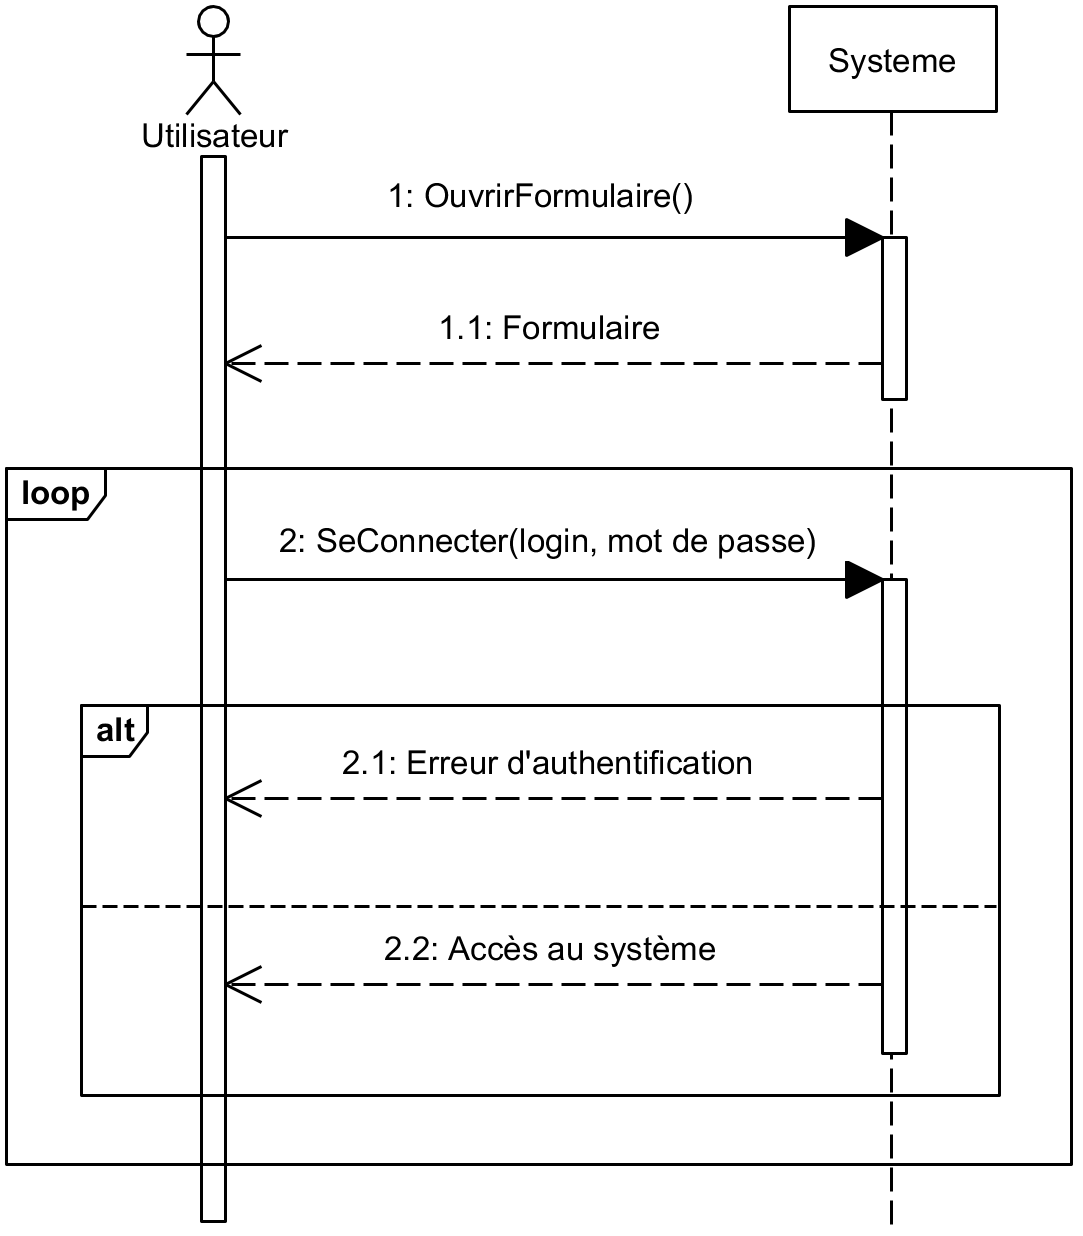
\includegraphics[width=90mm]{images/diagramme-de-sequence/sd-auth.png}
            \captionof{figure}{Diagramme de séquences S’authentifier}
            \label{fig:sdAuthentifier}
        \end{figure}
    \subsubsection[Afficher avis]{Afficher avis}
        \begin{figure}[H]
            \centering
            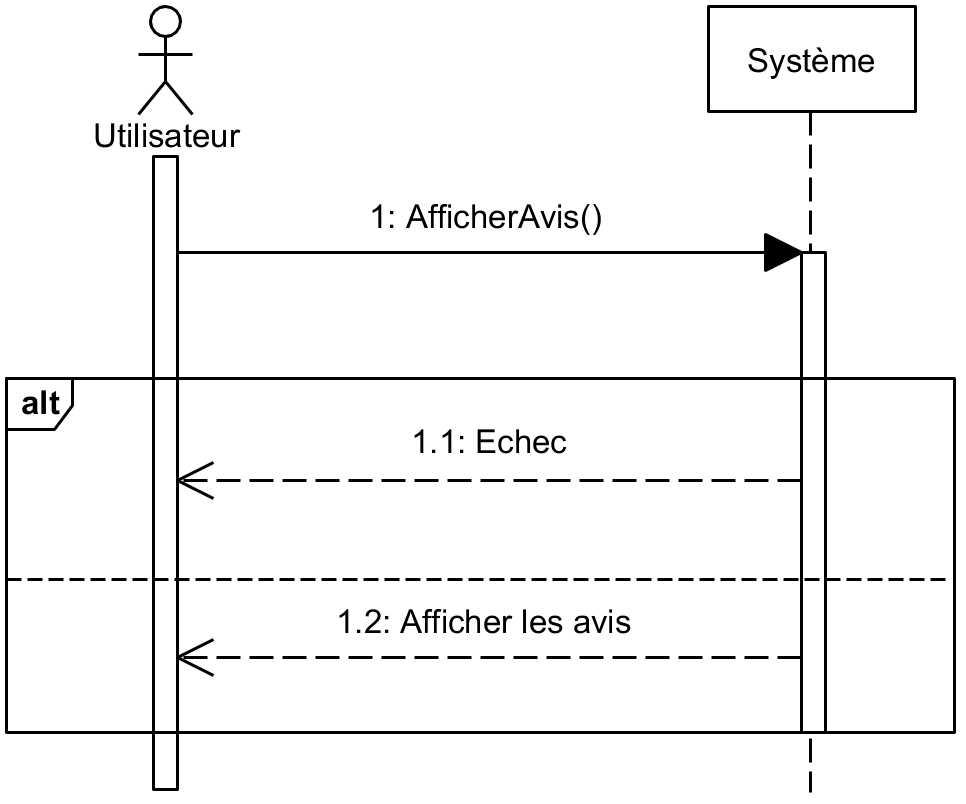
\includegraphics[width=90mm]{images/diagramme-de-sequence/sd-afficher-avis.png}
            \captionof{figure}{Diagramme de séquences Afficher avis}
            \label{fig:sdAffavis}
        \end{figure}
\pagebreak
    \subsubsection[Scanner ticket]{Scanner ticket}
        \begin{figure}[H]
            \centering
            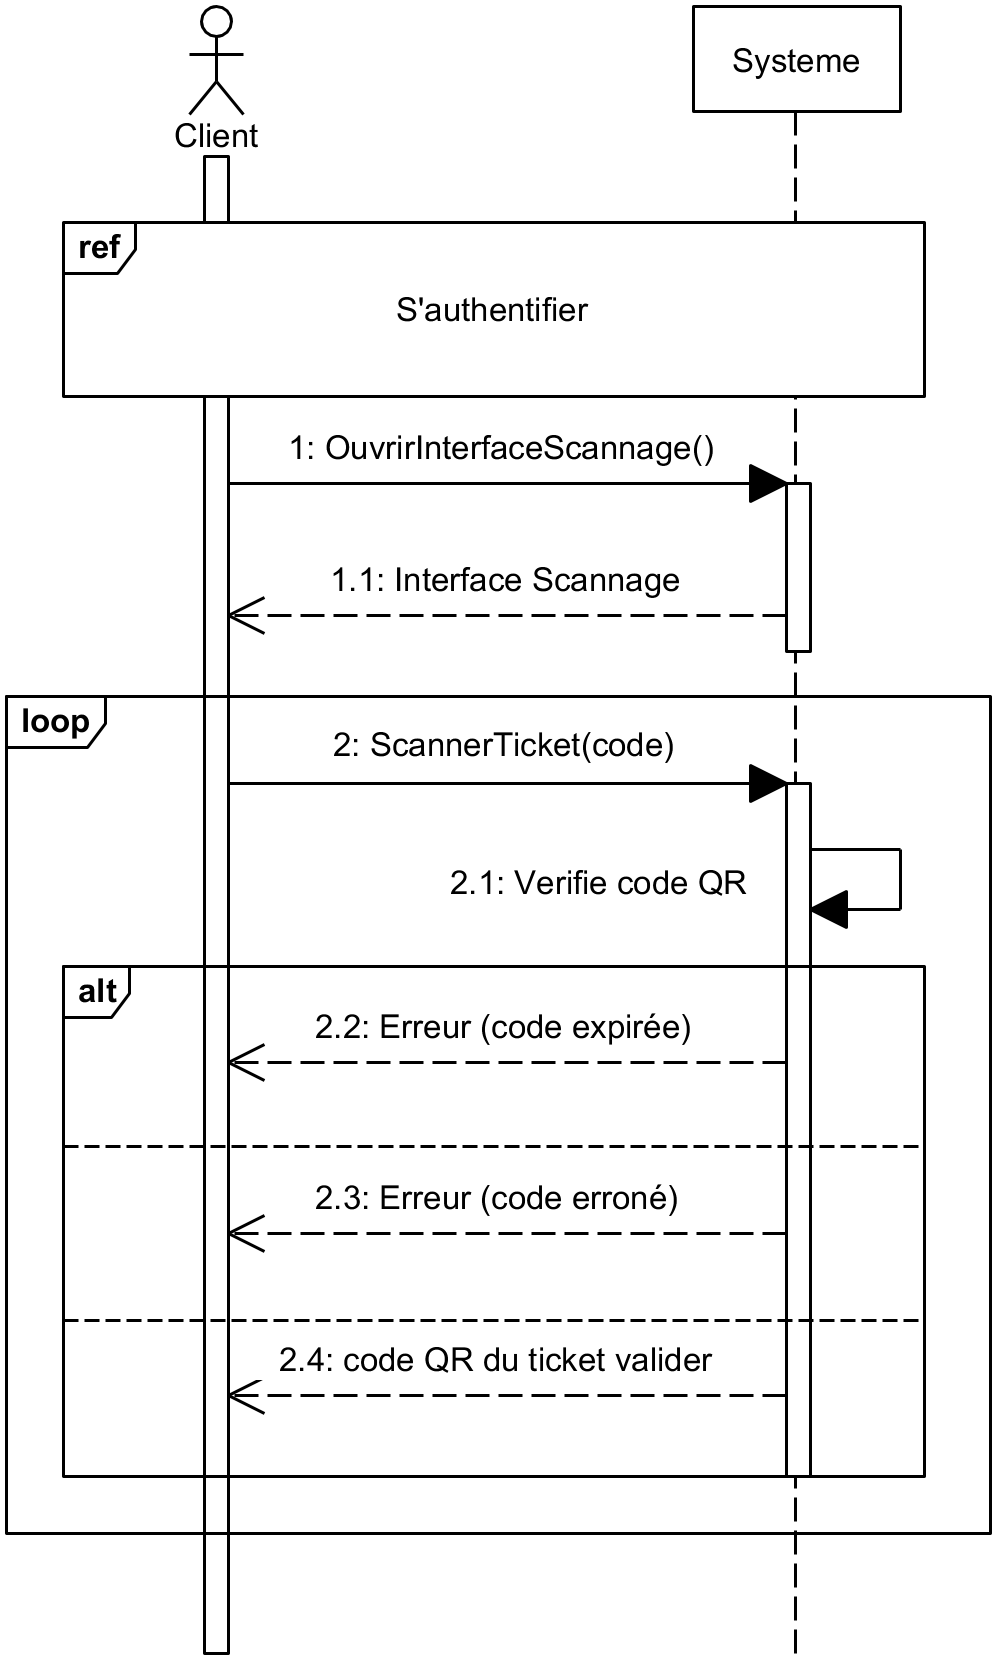
\includegraphics[width=100mm]{images/diagramme-de-sequence/sd-scanner.png}
            \captionof{figure}{Diagramme de séquences Scanner ticket}
            \label{fig:sdScannerTicket}
        \end{figure}
\pagebreak
    \subsubsection[Afficher notification]{Afficher notification}
        \begin{figure}[H]
            \centering
            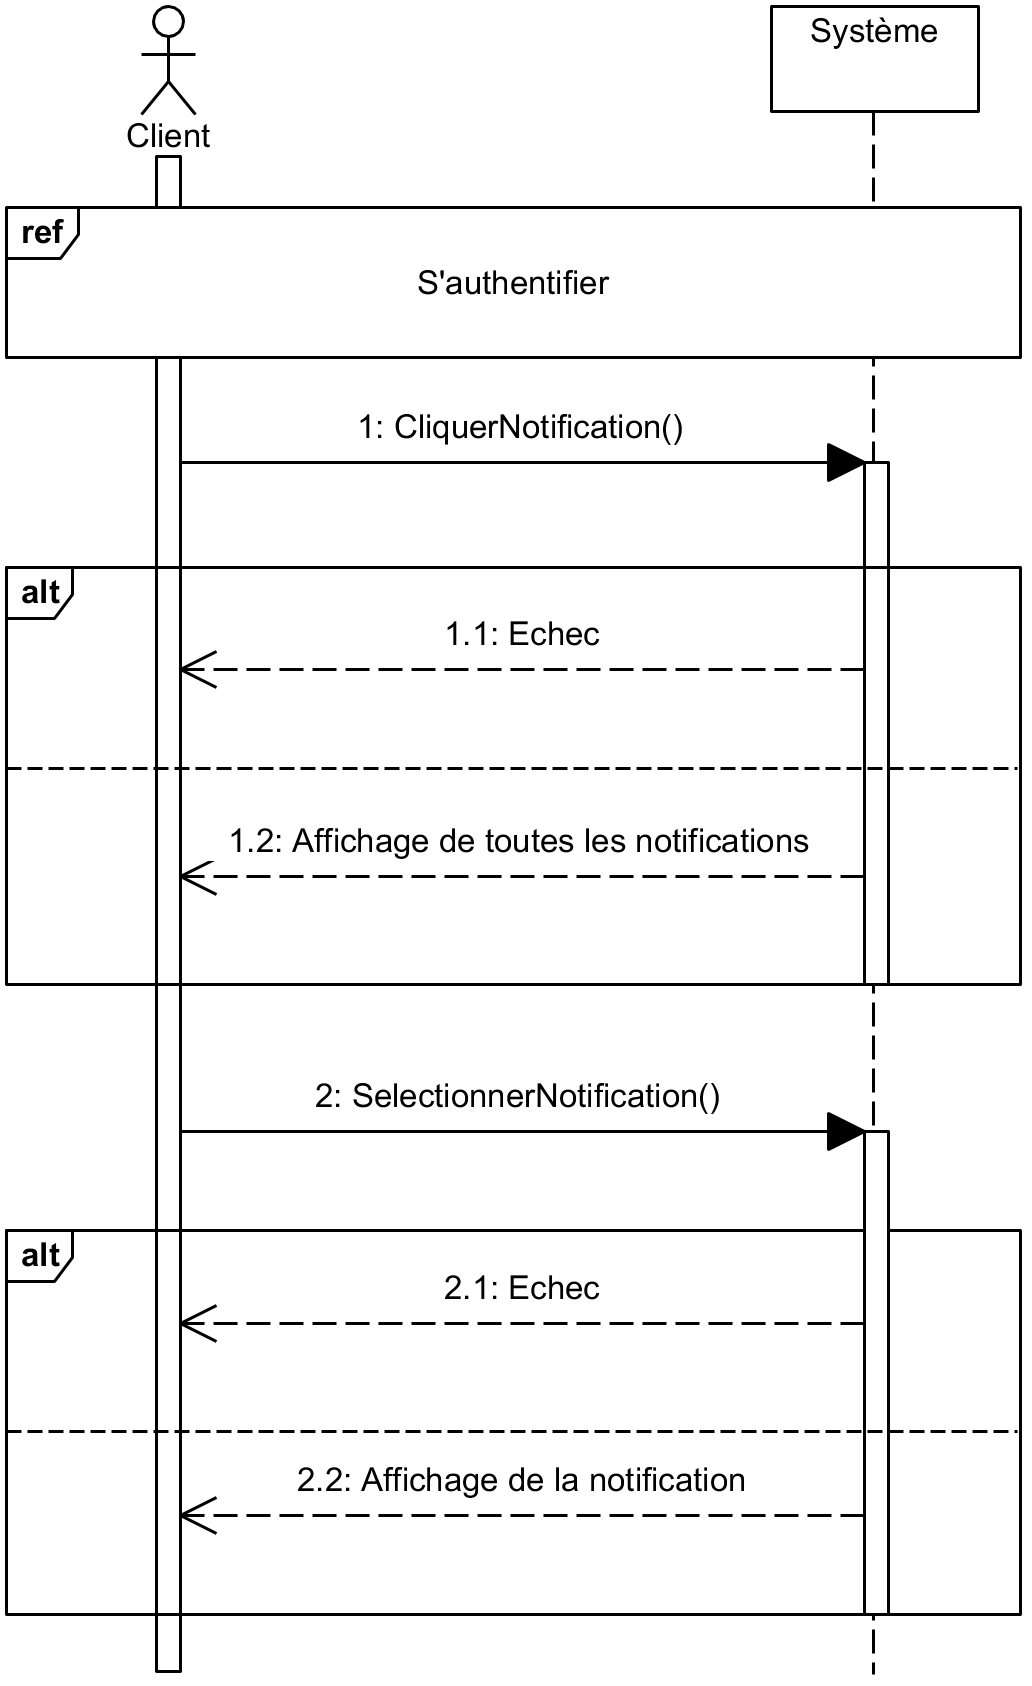
\includegraphics[width=100mm]{images/diagramme-de-sequence/sd-notification.png}
            \captionof{figure}{Diagramme de séquences Afficher notification}
            \label{fig:sdAffNotification}
        \end{figure}
\pagebreak
    \subsubsection[Donner avis]{Donner avis}
        \begin{figure}[H]
            \centering
            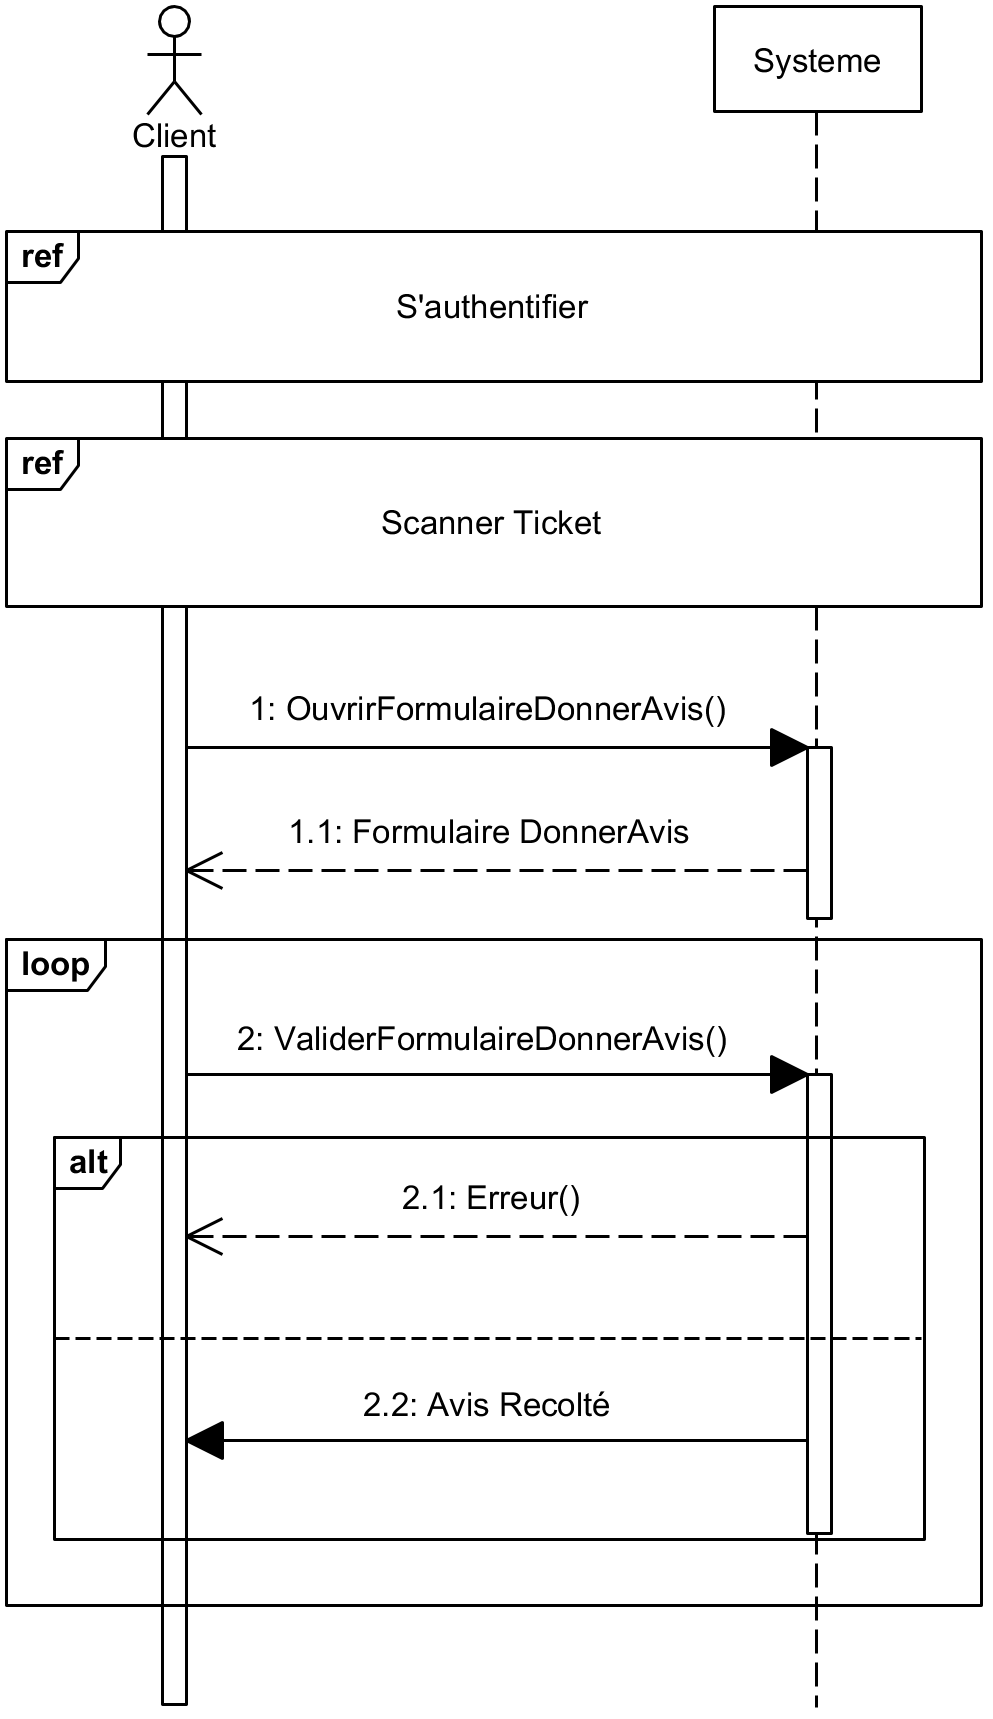
\includegraphics[width=100mm]{images/diagramme-de-sequence/sd-donner-avis.png}
            \captionof{figure}{Diagramme de séquences Donner Avis}
            \label{fig:sdDonnerAvis}
        \end{figure}
\pagebreak
    \subsubsection[Vendre ticket]{Vendre ticket}
        \begin{figure}[H]
            \centering
            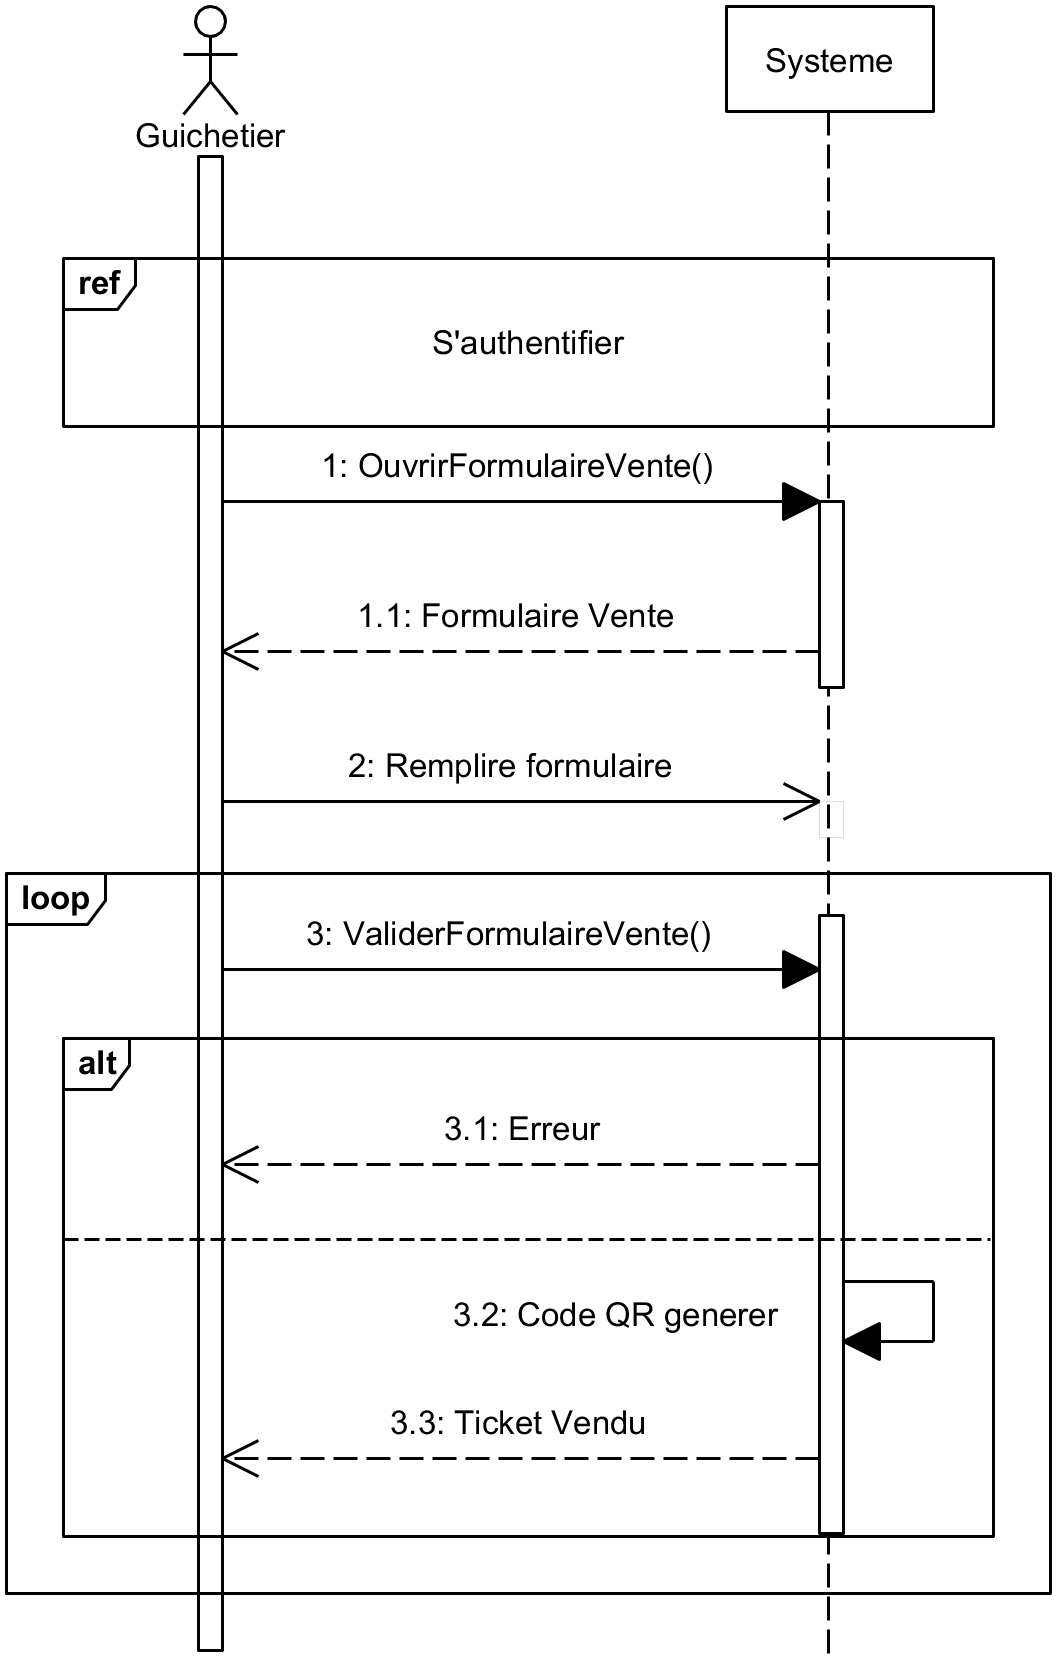
\includegraphics[width=100mm]{images/diagramme-de-sequence/sd-vendre-ticket.png}
            \captionof{figure}{Diagramme de séquences Vendre ticket}
            \label{fig:sdVendreTicket}
        \end{figure}
\pagebreak
    \subsubsection[Générer tableau de bord]{Générer tableau de bord}
        \begin{figure}[H]
            \centering
            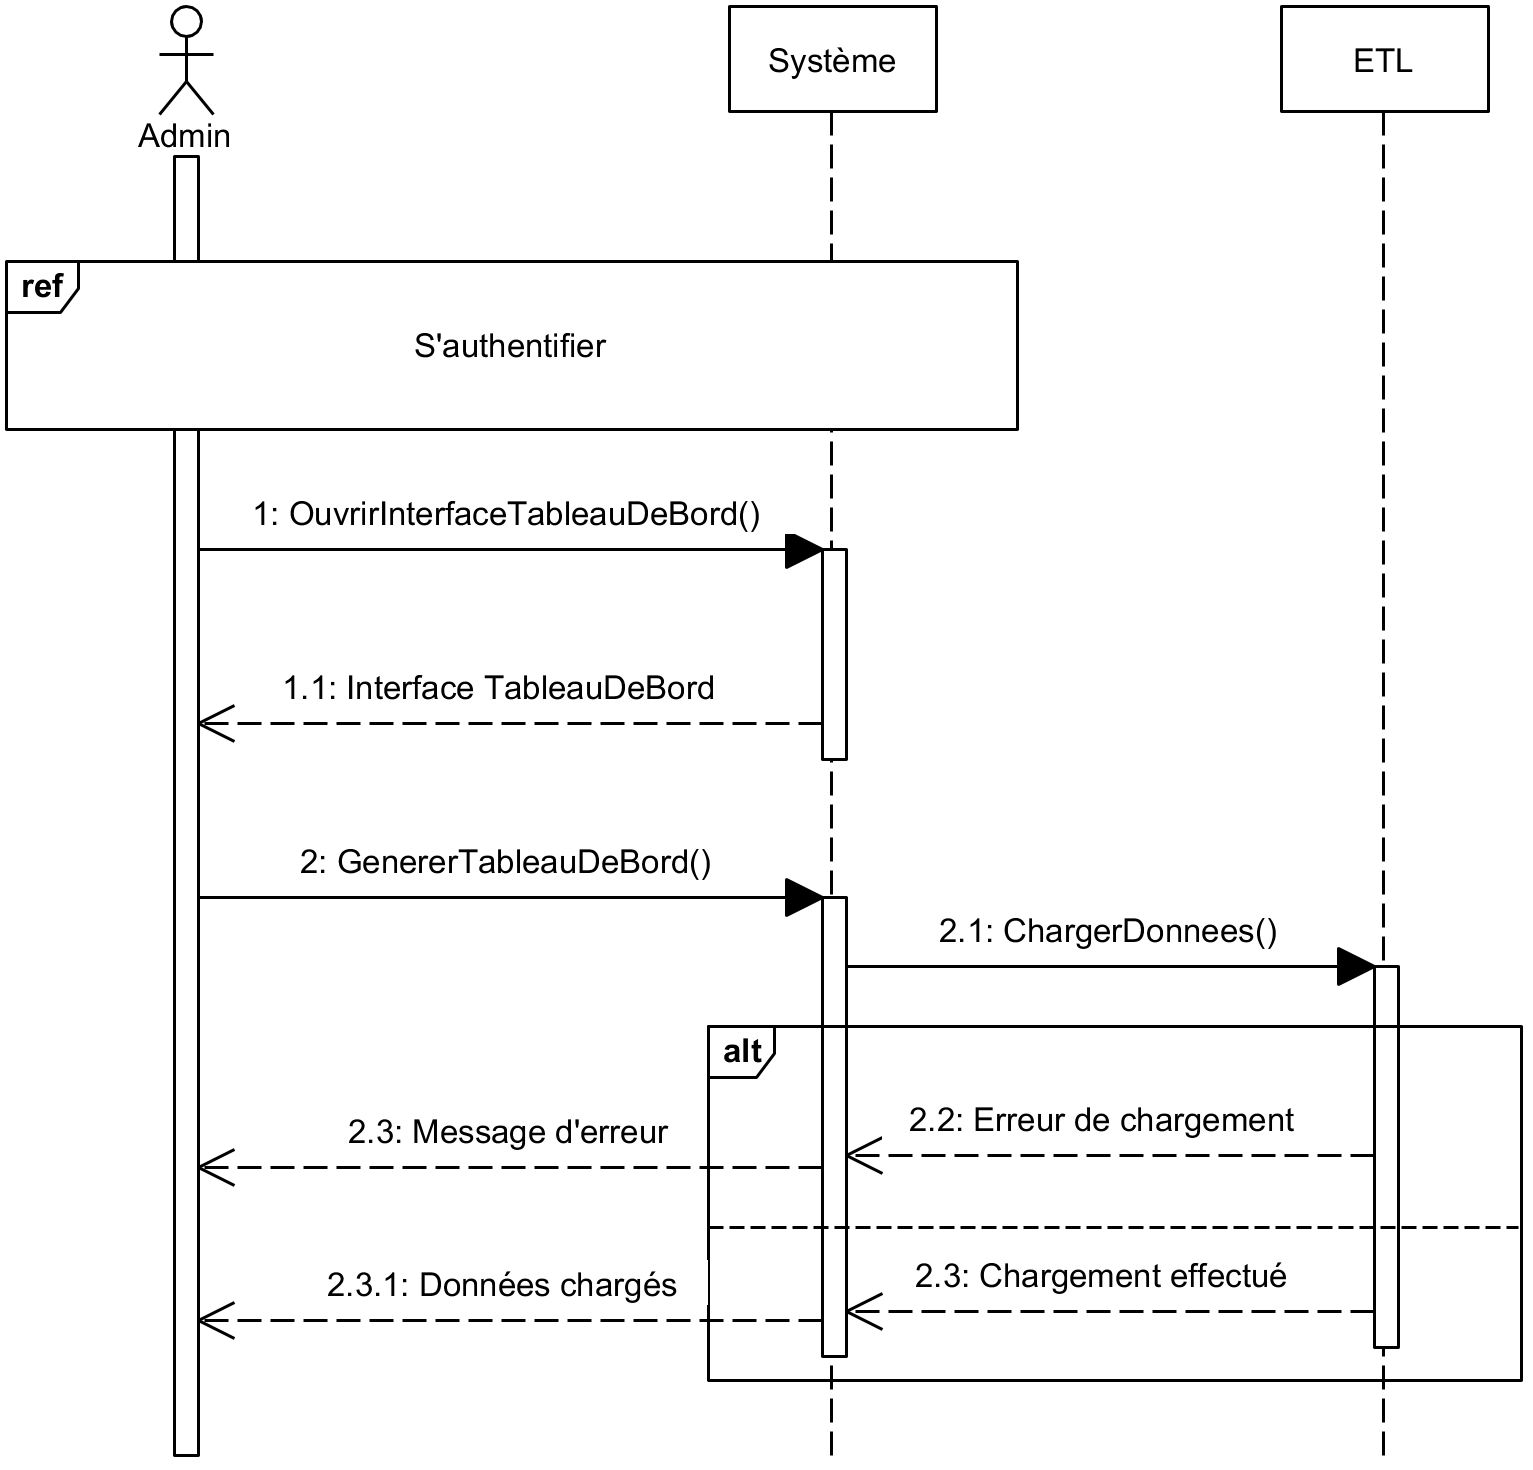
\includegraphics[width=130mm]{images/diagramme-de-sequence/sd-gene-dashboard.png}
            \captionof{figure}{Diagramme de séquences Générer tableau de bord}
            \label{fig:sdGenTab}
        \end{figure}
\pagebreak
    \subsubsection[Créer compte]{Créer compte}
        \begin{figure}[H]
            \centering
            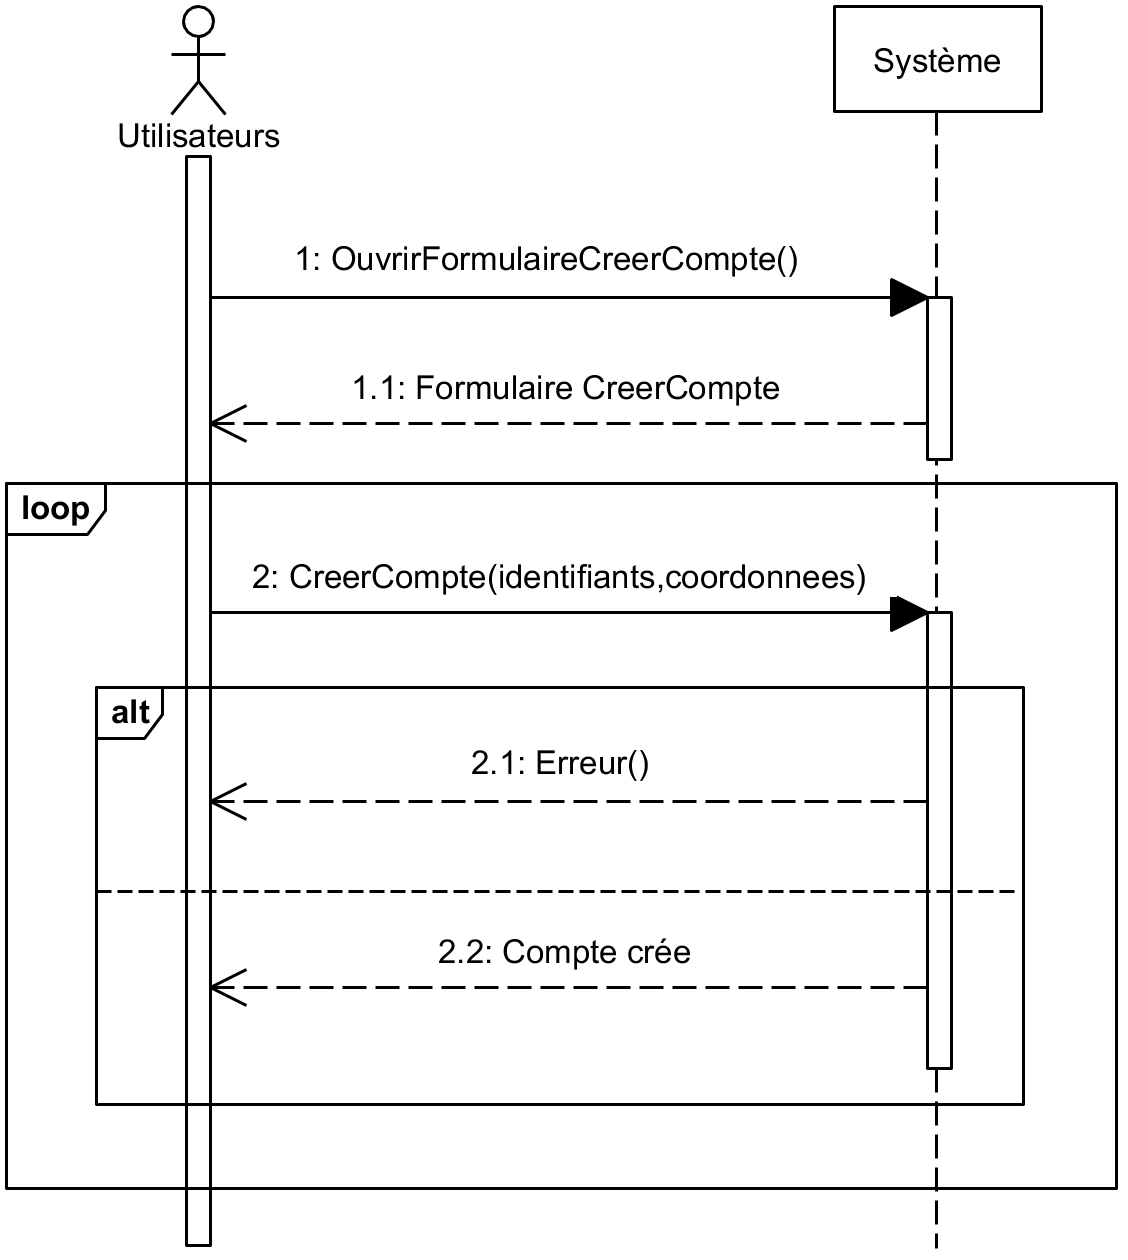
\includegraphics[width=90mm]{images/diagramme-de-sequence/sd-compte.png}
            \captionof{figure}{Diagramme de séquences Créer compte}
            \label{fig:sdCreerCompte}
        \end{figure}
    \subsubsection[Consulter tableau de bord]{Consulter tableau de bord}
        \begin{figure}[H]
            \centering
            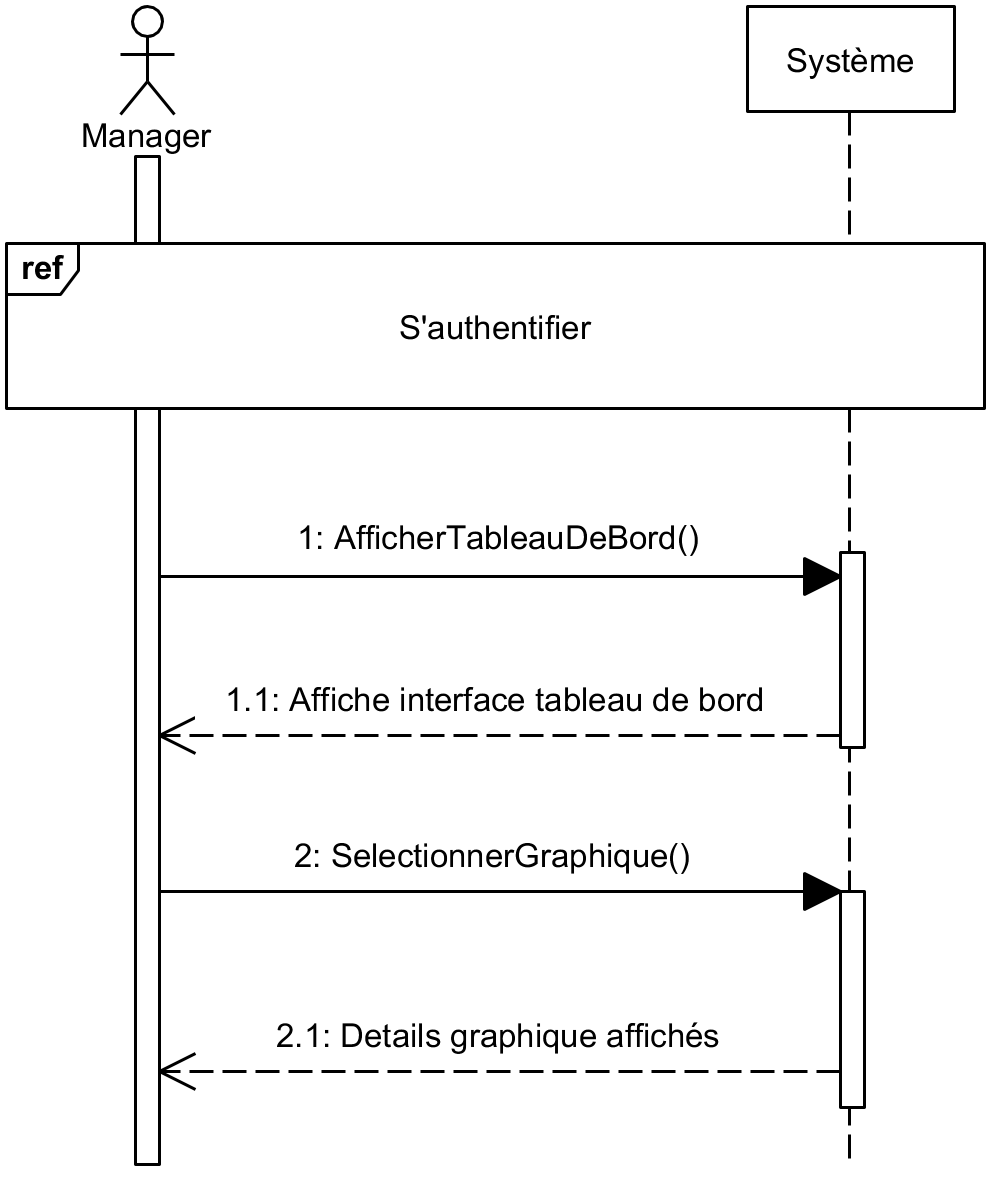
\includegraphics[width=80mm]{images/diagramme-de-sequence/sd-cons-dashboard.png}
            \captionof{figure}{Diagramme de séquences Consulter tableau de bord}
            \label{fig:sdConTab}
        \end{figure}
\pagebreak
    \subsubsection[Envoyer message]{Envoyer message}
        \begin{figure}[H]
            \centering
            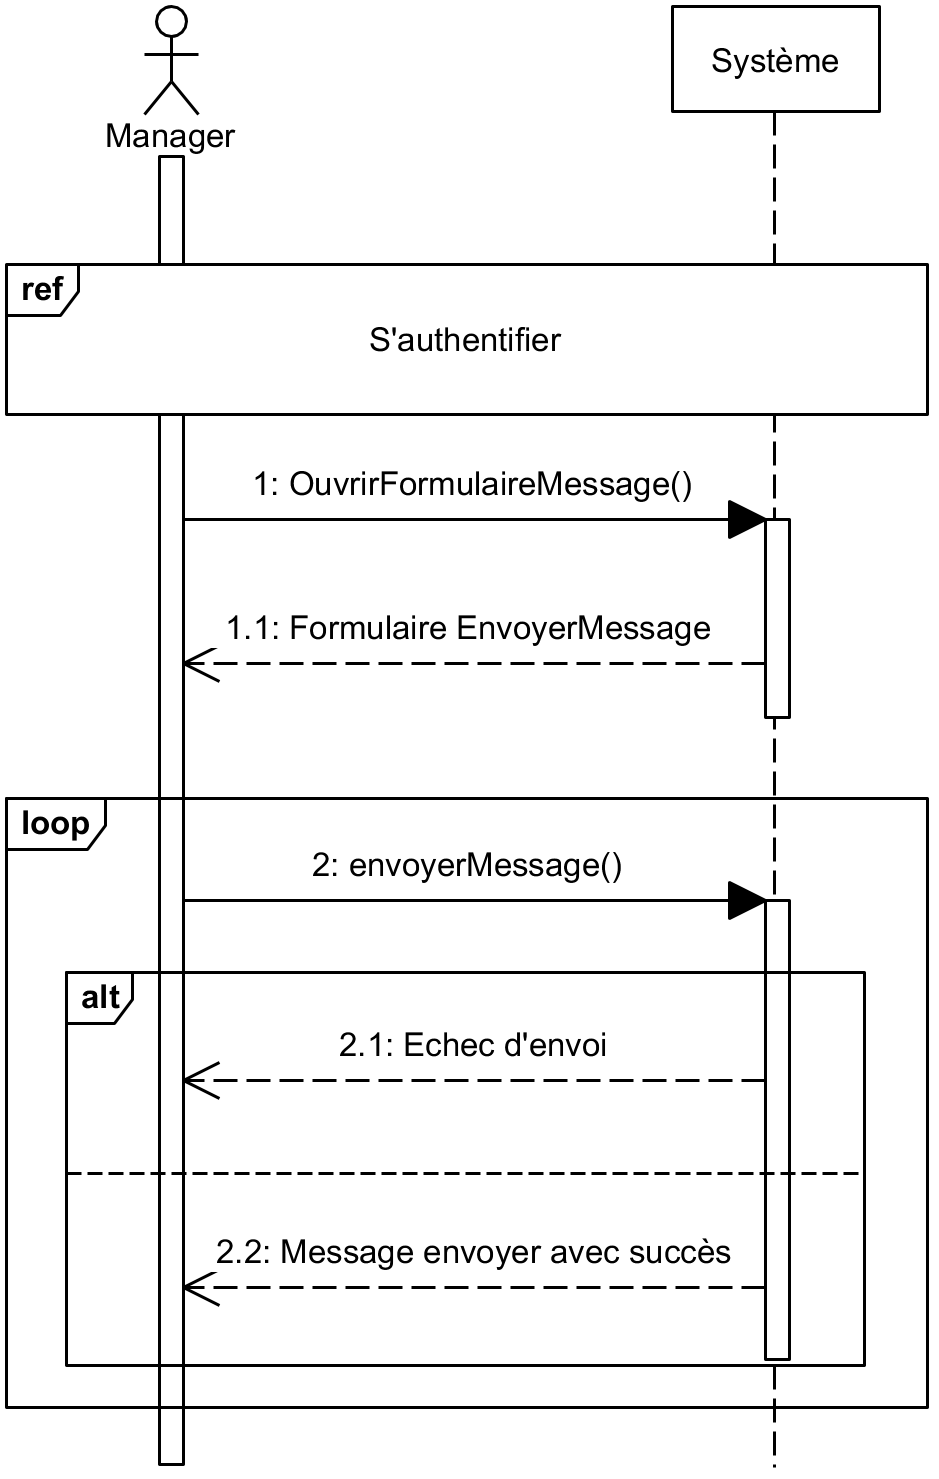
\includegraphics[width=100mm]{images/diagramme-de-sequence/sd-message.png}
            \captionof{figure}{Diagramme de séquences Envoyer message}
            \label{fig:sdSendSms}
        \end{figure}
        \section[Phase d’analyse]{Phase d’analyse}
    \subsection[Modèle du domaine]{Modèle du domaine}
    \subsection[Diagrammes de classes participantes]{Diagrammes de classes participantes}
        \subsubsection[Créer compte]{Créer compte}
        \subsubsection[S’authentifier]{S’authentifier}
        \subsubsection[Consulter avis]{Consulter avis}
        \subsubsection[Afficher notification]{Afficher notification}
        \subsubsection[Scanner jeton]{Scanner jeton}
        \subsubsection[Donner avis]{Donner avis}
        \subsubsection[Établir rapport]{Établir rapport}
        \subsubsection[Vendre billet]{Vendre billet}
        \subsubsection[Gérer compte]{Gérer compte}
        \subsubsection[Ajouter évaluation]{Ajouter évaluation}
        \subsubsection[Générer tableau de bord]{Générer tableau de bord}
        \subsubsection[Consulter tableau de bord]{Consulter tableau de bord}
        \subsubsection[Consulter rapport]{Consulter rapport}
        \section[Phase de conception]{Phase de conception}
    \subsection[Diagramme de classes de conception]{Diagramme de classes de conception}
    \section[Conclusion partielle]{Conclusion partielle}